\documentclass{beamer}
\usetheme{Dresden}
\usecolortheme{orchid}

\usepackage[french]{babel}
\usepackage[utf8]{inputenc}
\usepackage[T1]{fontenc}
\usepackage{graphicx}
\usepackage{tikz}
\usepackage{fontawesome}
\usepackage{amsmath}

\graphicspath{{../report/ims/}{ims/}}

\title{Vérification de la perspective dans les peintures}
\subtitle{Stage de M1}
\date{4 Septembre 2019}
\author{
	Yoann Coudert--Osmont \inst{1} \and \\
	\textit{Encadré par} Elmar Eisemann \textit{et} Ricardo Marroqium \inst{2}
}
\institute{
	\inst{1} ENS de Lyon \and
	\inst{2} TU Delft
}

\begin{document}
	
	\begin{frame}
		\titlepage
	\end{frame}

	\section{Règles de perspective}

	\begin{frame}{Lignes et points de fuites}
		\centering
		\begin{figure}[h]
			\begin{tikzpicture}[thick]
			\draw[] (0, 0) -- (1, 0) -- (1, 1) -- (0, 1) -- cycle;
			\draw[red] (-2.5, 2.25) -- (6, 2.25);
			\draw[green] (0, 1) -- (0.8, 1.5);
			\draw[green, dashed] (0.8, 1.5) -- (2, 2.25);
			\draw[green] (1, 1) -- (1.4, 1.5);
			\draw[green, dashed] (1.4, 1.5) -- (2, 2.25);
			\draw (0.8, 1.5) -- (1.4, 1.5);
			\draw[green] (1, 0) -- (1.4, 0.9);
			\draw[green, dashed] (1.4, 0.9) -- (2, 2.25);
			\draw (1.4, 0.9) -- (1.4, 1.5);
			
			\node[blue] (VP) at (2, 2.25) {$\bullet$};
			\node[above, blue] at (2, 2.25) {\small Point de fuite};
			\node[below, red] at (5, 2.25) {\small Ligne de fuite};
			\node[left, green] at (0.4, 1.4) {\small Lignes parallèles};
			\end{tikzpicture}
			\caption{Illustration des règles de perspective}
		\end{figure}
	\end{frame}

	\begin{frame}
		\centering
		\begin{figure}[h]
			\begin{tikzpicture}[thick, yscale=0.65, xscale=0.82]
			\draw[very thick] (0, 6) -- (12, 6);
			\draw[semithick] (0, 0) -- (12, 0);
			\node[above] at (6, 6) {\small Ligne de fuite};
			\node[above, red] at (0, 6) {\small $A$};
			\node[above, blue] at (4, 6) {\small $B$};
			\node[above, green] at (12, 6) {\small $C$};
			
			\foreach \i in {2, ..., 11} \draw[red] (0, 6) -- (\i, 0);
			\foreach \i in {1.333, 2.666, ..., 9.333} \draw[blue] (4, 6) -- (\i, 0);
			
			\draw[red] (2, -0.3) node {\texttt{|}} -- node[below] {$d_A$} (3, -0.3) node {\texttt{|}};
			\draw[blue] (4, -0.3) node {\texttt{|}} -- node[below] {$d_B$} (5.333, -0.3) node {\texttt{|}};
			\draw[green] (6, -0.3) node {\texttt{|}} -- node[below] {$d_C$} (8, -0.3) node {\texttt{|}};
			
			\node[below, align=center] at (10.2, 0)
			{\footnotesize ligne parallèle à \\[-1mm]
				\footnotesize la ligne de fuite};
			
			\clip (0, 0) rectangle (12, 6);
			\foreach \i in {-4, -2, ..., 10} \draw[green] (12, 6) -- (\i, 0);
			\foreach \i in {4, 8, ..., 24} \draw[blue] (-12, 6) -- (\i, 0);
			\end{tikzpicture}
		\end{figure}
		$$ {\color{blue} B} = \dfrac{{\color{green} d_C} {\color{red} A} + {\color{red} d_A} {\color{green} C}}{{\color{red} d_A} + {\color{green} d_C}} \qquad {\color{blue} d_B} = 2 \dfrac{{\color{red} d_A} {\color{green} d_C}}{{\color{red} d_A} + {\color{green} d_C}} $$
	\end{frame}

	\section{Détection des lignes}
	
	\begin{frame}{Les étapes}
		\begin{itemize}
			\small \item Changement d'espace de couleurs (RGB $\rightarrow$ CIE Lab)
			\small \item Lissage / élimination du bruit
			\small \item Calcul du gradient
			\small \item Transformée de Hough
			\small \item Regroupement des lignes et calcul des points de fuites
		\end{itemize}
		\centering
		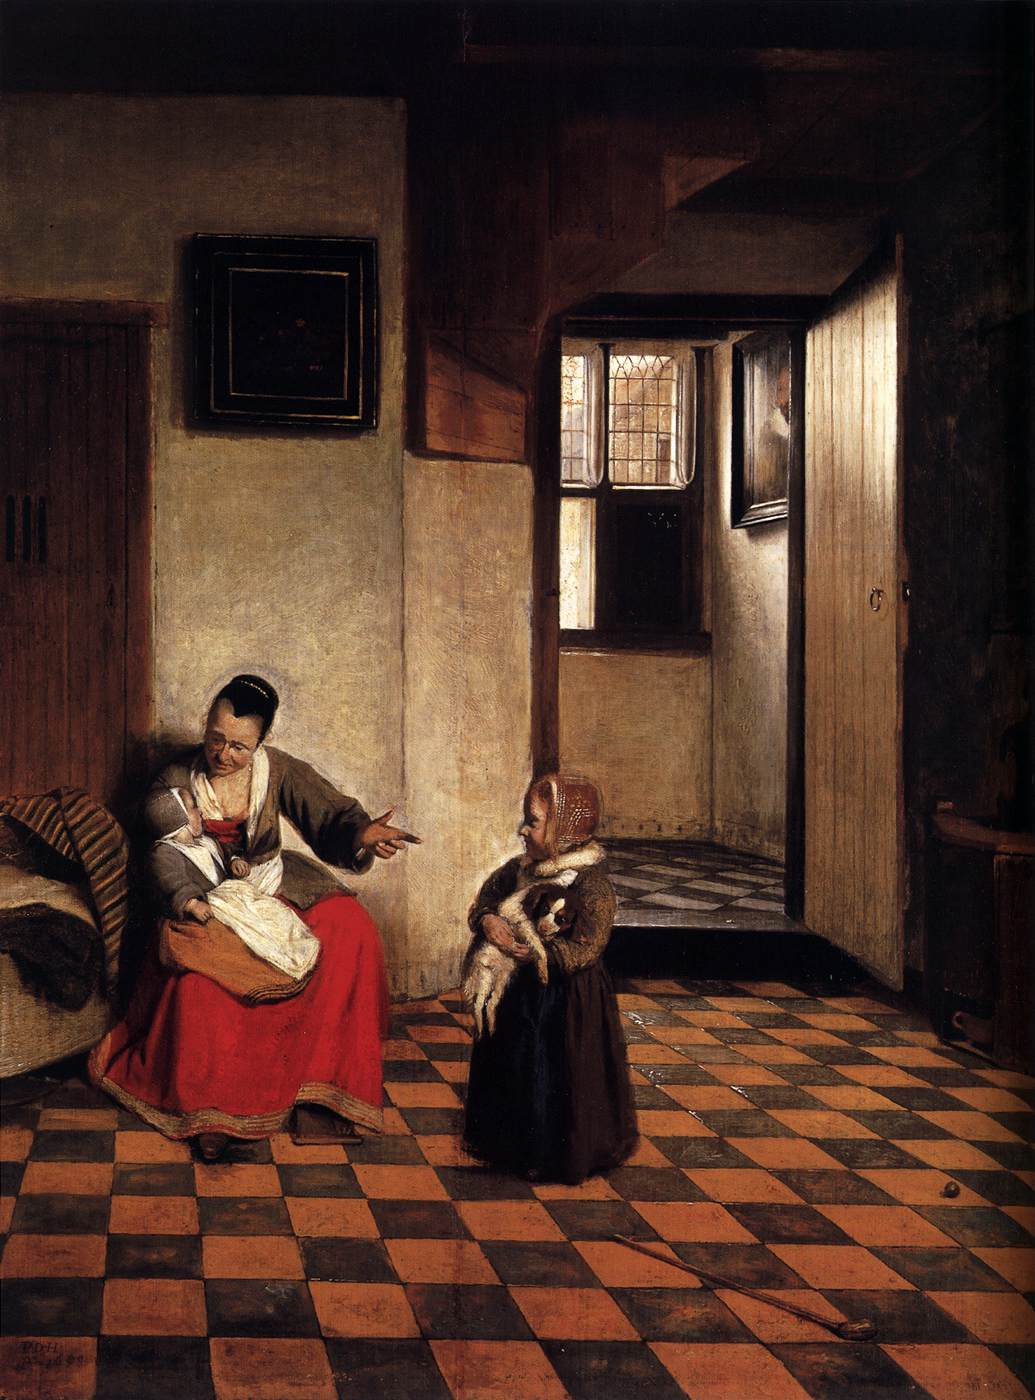
\includegraphics[scale=0.33]{hooch1.jpg}
		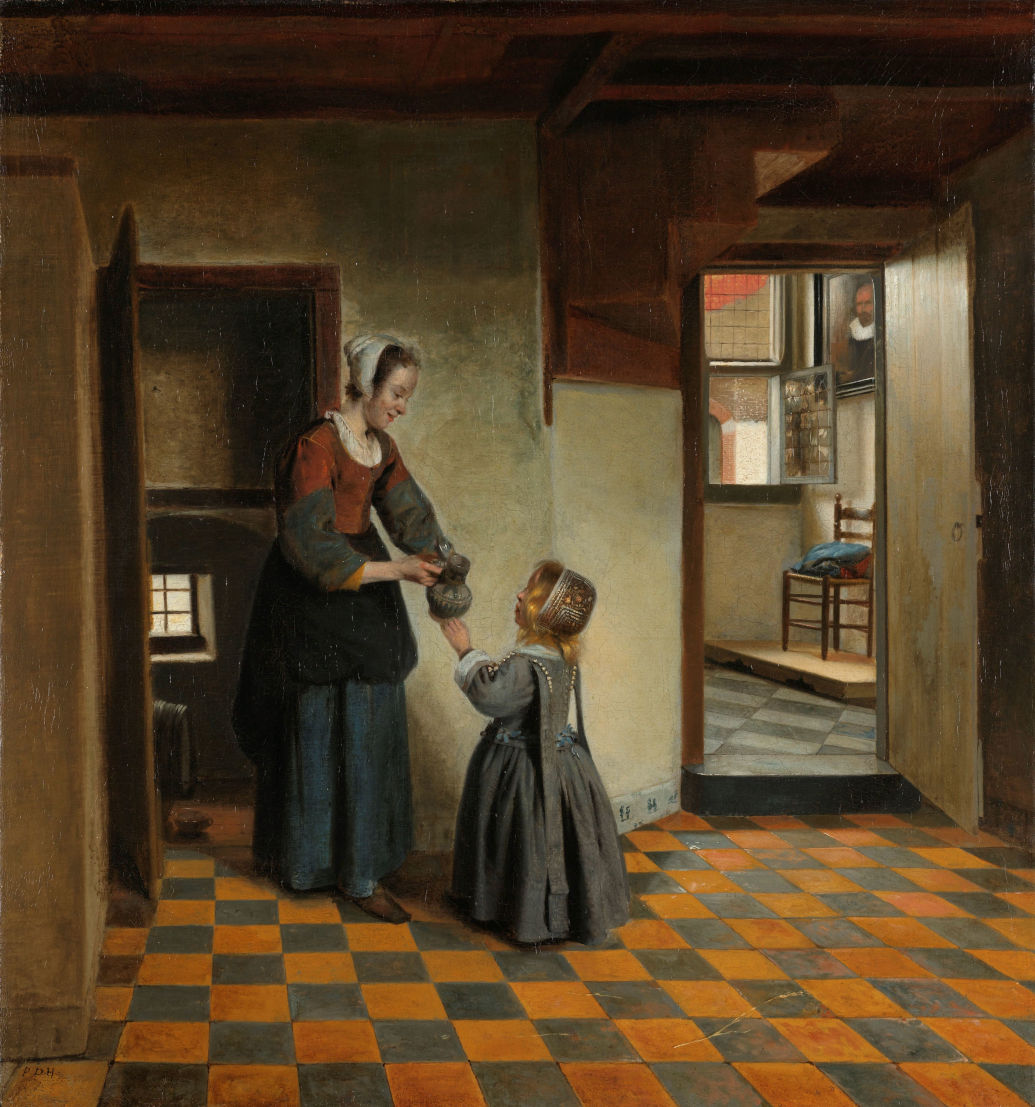
\includegraphics[scale=0.4]{hooch2.jpg}
	\end{frame}

	\begin{frame}{CIE Lab}
		Besoin d'un espace dans lequel la distance entre deux couleur est en accord avec l'œil humain :
		$$ \Delta E = \sqrt{(R_1 - R_2)^2 + (V_1 - V_2)^2 + (B_1 - B_2)^2} \qquad \huge \color{red} \text{\faThumbsODown} $$
		$$ \Delta E = \sqrt{(L_1^* - L_2^*)^2 + (a_1^* - a_2^*)^2 + (b_1^* - b_2^*)^2} \qquad \huge \color{green} \text{\faThumbsOUp}  $$
	\end{frame}
	
	\begin{frame}{Filtre gaussien}
		\centering
		\begin{tikzpicture}[scale=0.8]
		\node at (0, 0.9) {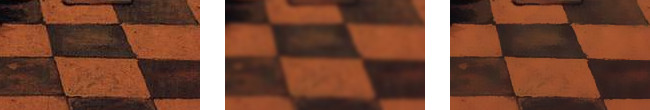
\includegraphics[width=8cm]{smoothing.jpg}};
		\node[below] at (0, 0) {\small Filtre gaussien};
		\node[below] at (-3.45, 0) {\small Image original};
		\fill[white] (1.7, 0) rectangle (5.1, 2);
		\fill[white] (-5.1, 0) rectangle (-8.6, 2);
		\end{tikzpicture}
		$$ I'(z) = \dfrac{1}{W} \sum_{z' \in \Omega_{z}} I(z') \exp \left( - \dfrac{\| z - z'\|^2}{2 \sigma^2} \right) $$
		\small Où $\Omega_{z}$ est une fenêtre autour de $z \in \N^2$ et $W = \sum_{z' \in \Omega_{z}} \exp \left( - \frac{\| z - z'\|^2}{2 \sigma^2} \right)$.
	\end{frame}

	\begin{frame}{Filtre bilatéral}
		\centering
		\begin{tikzpicture}[scale=0.8]
		\node at (0, 0.9) {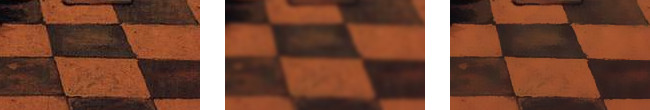
\includegraphics[width=8cm]{smoothing.jpg}};
		\node[below] at (0, 0) {\small Filtre gaussien};
		\node[below] at (-3.45, 0) {\small Image original};
		\node[below] at (3.45, 0) {\small Filtre Bilatéral};
		\end{tikzpicture}
		$$ I'(z) = \dfrac{1}{W} \sum_{z' \in \Omega_{z}} I(z) \, f(z, z') \, g \left( I(z), I(z') \right) $$
		\small Où $\Omega_{z}$ est une fenêtre autour de $z$ et $W = \sum_{z' \in \Omega_{z}} f(z, z') g(I(z), I(z'))$.
		$$ f(z, z') = \exp \left( - \dfrac{\| z - z'\|^2}{2 \sigma_f^2} \right) \qquad g(u, u') = \exp \left( - \dfrac{\| u - u'\|^2}{2 \sigma_g^2} \right) $$
	\end{frame}

	\begin{frame}{Sélection de zone intéressante}
		\begin{figure}[h]
			\centering
			\begin{tikzpicture}[scale=0.75]
			\node (a) at (0, 0) {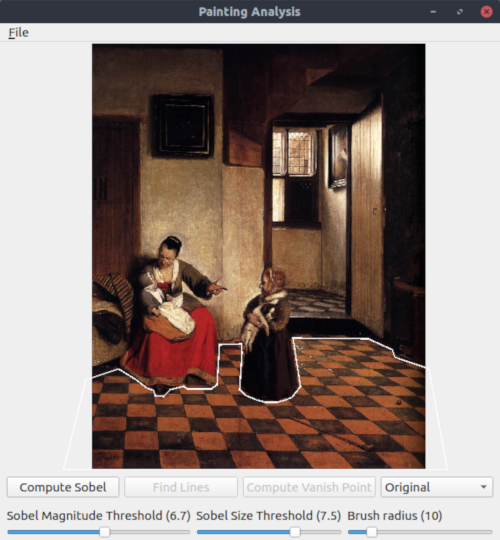
\includegraphics[scale=0.75]{zone_select.png}};
			\node (b) at (8.5, 0) {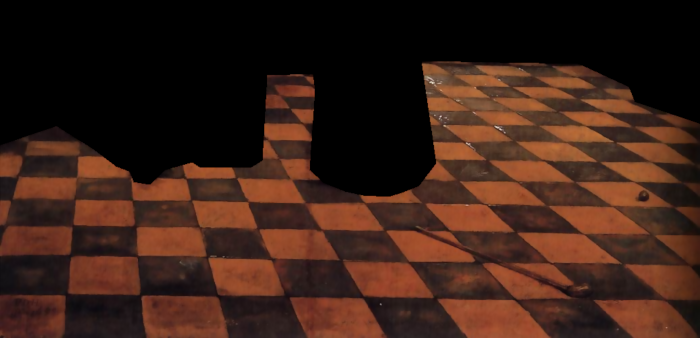
\includegraphics[scale=0.9]{bilateral.png}};
			\draw[->, ultra thick] (a) -- node[above, align=center]
			{\footnotesize Coupe et \\[-1mm]
				\footnotesize application du \\[-1mm]
				\footnotesize filtre bilatéral} (b);
			\end{tikzpicture}
		\end{figure}
	\end{frame}

\end{document}